\documentclass[11pt,a4paper]{article}

% ----- Packages -----
\usepackage[utf8]{inputenc}
\usepackage[T1]{fontenc}
\usepackage[margin=2.5cm]{geometry}
\usepackage{booktabs}
\usepackage{amsmath}
\usepackage{graphicx}
\usepackage{microtype}
\usepackage{hyperref}
\usepackage{float}
\usepackage{xcolor}
\usepackage{caption}
\usepackage{subcaption}
\captionsetup{font=small,labelfont=bf}

\hypersetup{
    colorlinks=true,
    linkcolor=blue,
    citecolor=blue,
    urlcolor=blue
}

\title{\textbf{CENG 467 -- Natural Language Understanding and Generation}\\[0.4em]
\Large Take-Home Midterm Examination}
\author{Enes Ergün Ho{\c s}gör\\Student ID: 300201053\\\small Repository: \url{https://github.com/hosgorenes/ceng467-takehome-midterm}}
\date{7 May 2026}

\begin{document}

\maketitle
\vspace{-0.4em}
\noindent\textit{All experiments use fixed train/validation/test splits and random seed 42. Test sets are reserved for final evaluation only.}
\vspace{0.4em}
\tableofcontents
\newpage

%==============================================================================
\section{Question 1: Representation Learning in Text Classification}
%==============================================================================

\subsection{Dataset and Preprocessing}
The IMDb Large Movie Review dataset~\cite{maas2011learning} is a binary sentiment benchmark of 50{,}000 reviews, balanced 50/50 across positive and negative labels and split equally between train and test (25{,}000 each). The training set was further partitioned with a 20\% held-out validation fraction, yielding 20{,}000 training and 5{,}000 validation examples. Reviews vary substantially in length, vocabulary register and topical focus.

A common pipeline strips HTML markup, lowercases text, and applies whitespace normalization. Stopword removal was deliberately omitted because negation words such as \emph{not}, \emph{never} and \emph{hardly} carry critical sentiment polarity. For the TF-IDF pipeline, two tokenization strategies were evaluated: a 30k-feature unigram vocabulary and a 50k-feature unigram+bigram vocabulary, both with sublinear TF scaling. The BiLSTM uses a 30k-type vocabulary with sequences padded/truncated to 256 tokens; the OOV rate is 3--5\% on the test set. DistilBERT applies its native WordPiece tokenizer, which virtually eliminates OOV tokens.

\subsection{Models}
\textbf{TF-IDF + Logistic Regression.} Sparse $n$-gram representation with sublinear TF scaling and L2 regularization ($C{=}1.0$). Two configurations: unigrams (30k features) and unigram+bigram (50k features).

\textbf{BiLSTM.} 128-dim embedding $\rightarrow$ 2 stacked BiLSTM layers (hidden 256/direction) $\rightarrow$ global temporal max-pool $\rightarrow$ dropout 0.3 $\rightarrow$ sigmoid head. Trained for 5 epochs (Adam, lr $10^{-3}$, batch 64, gradient clip 1.0).

\textbf{DistilBERT.} The \texttt{distilbert-base-uncased} checkpoint~\cite{sanh2019distilbert} is fine-tuned end-to-end with a linear head on the \texttt{[CLS]} representation: 3 epochs, AdamW, lr $2{\times}10^{-5}$, batch 16, 10\% linear warmup.

\subsection{Results}

\begin{table}[H]
\centering
\caption{Q1 Sentiment Classification -- IMDb test set (25{,}000 samples).}
\label{tab:q1}
\begin{tabular}{lcc}
\toprule
\textbf{Model} & \textbf{Accuracy} & \textbf{Macro-F1} \\
\midrule
TF-IDF + LR (unigram) & 0.8894 & 0.8894 \\
TF-IDF + LR (bigram)  & 0.8974 & 0.8974 \\
BiLSTM (2L, hid=256, dp=0.3) & 0.8327 & 0.8326 \\
DistilBERT (fine-tuned, 3 ep) & \textbf{0.9116} & \textbf{0.9116} \\
\bottomrule
\end{tabular}
\end{table}

\begin{figure}[H]
\centering
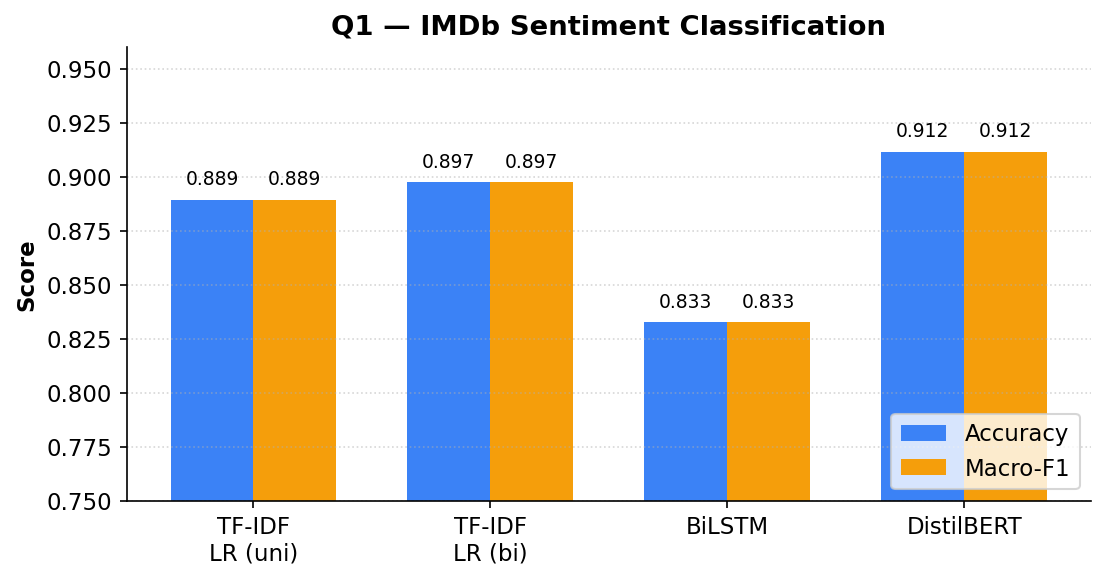
\includegraphics[width=0.78\textwidth]{figures/q1_comparison.png}
\caption{Accuracy and Macro-F1 across the four IMDb classifiers. DistilBERT leads, followed by the bigram TF-IDF baseline.}
\label{fig:q1_bar}
\end{figure}

\begin{figure}[H]
\centering
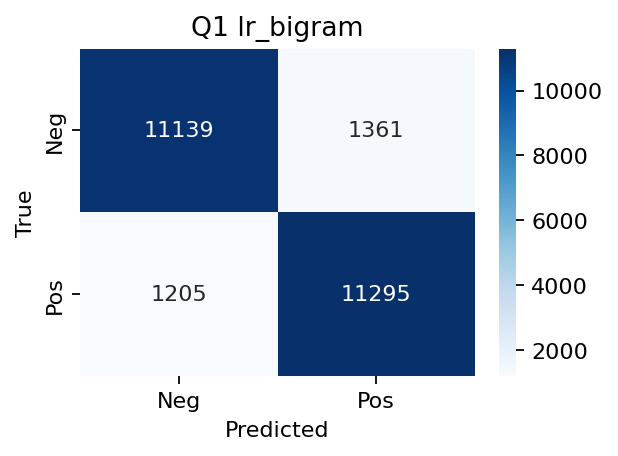
\includegraphics[width=0.32\textwidth]{figures/cm_lr_bigram.png}
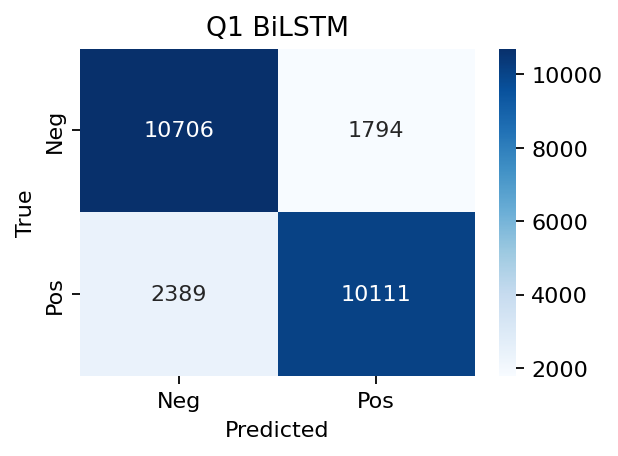
\includegraphics[width=0.32\textwidth]{figures/cm_bilstm.png}
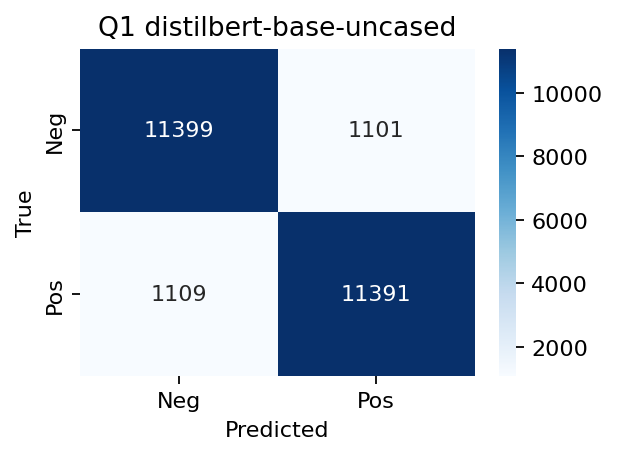
\includegraphics[width=0.32\textwidth]{figures/cm_distilbert.png}
\caption{Confusion matrices for TF-IDF+LR bigram (left), BiLSTM (centre), and DistilBERT (right). DistilBERT exhibits the most balanced error profile, while BiLSTM produces the largest absolute number of false positives and false negatives.}
\label{fig:q1_cm}
\end{figure}

\begin{figure}[H]
\centering
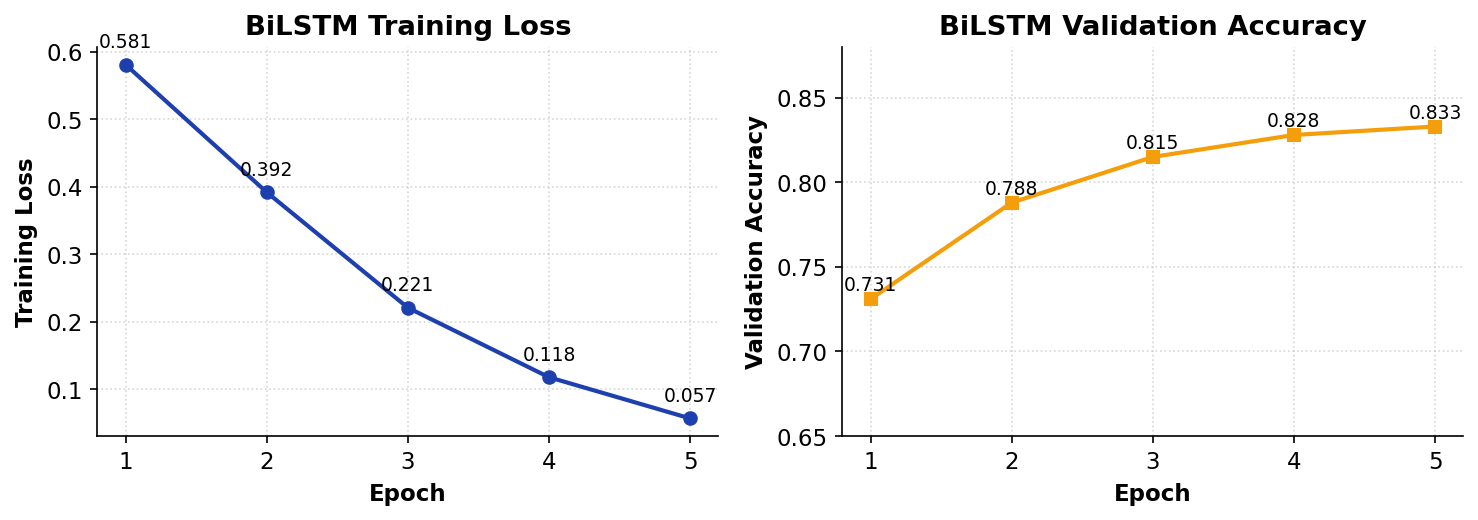
\includegraphics[width=0.92\textwidth]{figures/q1_bilstm_curves.png}
\caption{BiLSTM training dynamics over five epochs. Training loss decreases monotonically while validation accuracy plateaus near 0.83, a signal of mild overfitting consistent with the limited training-data regime.}
\label{fig:q1_curves}
\end{figure}

\begin{figure}[H]
\centering
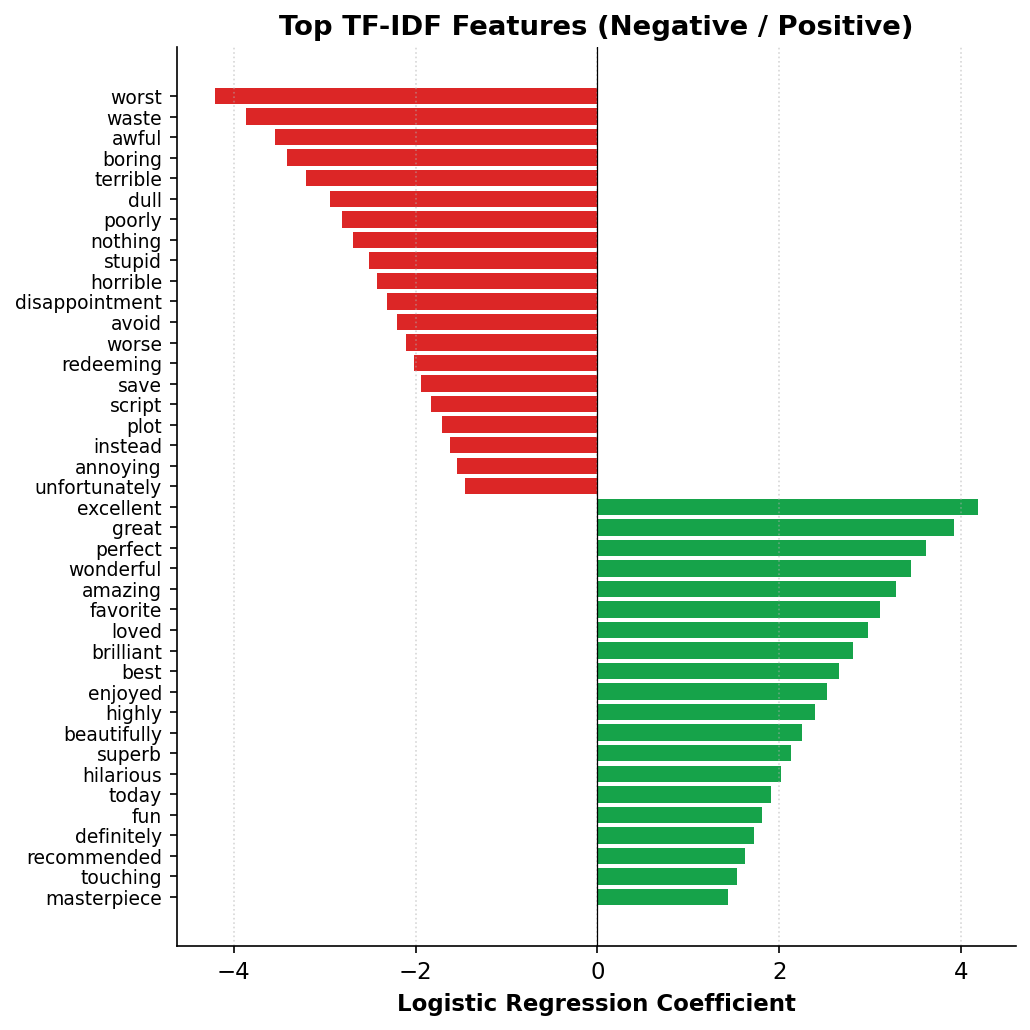
\includegraphics[width=0.62\textwidth]{figures/q1_feature_weights.png}
\caption{Top 20 negative (red) and positive (green) TF-IDF unigram features ranked by Logistic Regression coefficient magnitude. Each weight is directly interpretable as the global contribution of that token to the predicted class.}
\label{fig:q1_features}
\end{figure}

DistilBERT achieves the highest accuracy (91.16\%) and Macro-F1 (91.16\%), beating the closest competitor by at least 1.4 points. The bigram TF-IDF model is a remarkably strong baseline at 89.74\%, confirming that sparse $n$-gram features capture substantial sentiment signal in a task where bag-of-phrases is nearly sufficient. The BiLSTM underperforms both TF-IDF variants -- counterintuitive at first glance, but explainable by data efficiency: training expressive recurrent embeddings from scratch on 20k examples is a fragile regime, as visible in Figure~\ref{fig:q1_curves} where validation accuracy plateaus while training loss continues to drop.

\subsection{Error Analysis}
Misclassifications cluster around five recurring linguistic patterns. (i) \emph{Qualified praise / irony} -- example index 4 (``If you haven't enjoyed a Van Damme movie since Bloodsport, you probably will not like this'') is misread as positive by all three models because positive-valence words dominate local aggregation while the global verdict is negative. (ii) \emph{Genre-specific superlatives} -- example index 6 (martial-arts review) confuses the BiLSTM by activating positive neurons on words like ``best'' and ``classics'' even when the discourse trajectory is mixed. (iii) \emph{Sharp polarity shifts} -- example index 23 (``disguised as a thinker's film $\dots$ utter pretentious crap'') defeats the unigram TF-IDF model because positive tokens in the first half numerically outweigh the late negative pivot. (iv) \emph{Conditional endorsements} -- ``if you like this genre, you'll enjoy it'' is pragmatically negative when written by a reviewer who dislikes the genre. (v) \emph{Information-sparse short reviews} drive all models towards near-chance predictions.

\subsection{Discussion}
The performance ordering -- DistilBERT $>$ TF-IDF (bigram) $>$ TF-IDF (unigram) $>$ BiLSTM -- reflects three theoretically grounded effects. First, document-level sentiment is partially \emph{order-insensitive}: the distribution of opinion words is often sufficient to determine polarity, which is why TF-IDF baselines remain competitive. Second, the BiLSTM's deficit is a \emph{data-efficiency} problem rather than an architectural one: starting from random embeddings on 20k samples is too little signal to learn a useful representation geometry; pre-trained word vectors (GloVe/fastText) would close most of this gap. Third, DistilBERT's advantage is a direct consequence of \emph{transfer learning}: a contextual embedding space already encodes much of the syntactic/semantic structure required for sentiment, so fine-tuning only adapts the top layers. This advantage costs roughly two orders of magnitude in inference latency, creating a real accuracy/latency trade-off: at high request volumes the bigram TF-IDF model is a Pareto-attractive choice.

%==============================================================================
\section{Question 2: Named Entity Recognition}
%==============================================================================

\subsection{Dataset and BIO Alignment}
The CoNLL-2003 dataset~\cite{tjong2003introduction} is the canonical English NER benchmark, derived from Reuters newswire and annotated under the BIO scheme for four entity types: persons (PER), organizations (ORG), locations (LOC) and miscellaneous (MISC). The training, validation and test splits contain $\sim$14{,}987 / 3{,}466 / 3{,}684 sentences. Approximately 83\% of tokens carry the \texttt{O} label, which makes entity-level Precision/Recall/F1 -- not token-level accuracy -- the appropriate metrics. For BERT, when WordPiece splits a word into multiple subword pieces, only the first piece carries the gold label; subsequent pieces receive an ignore index of $-100$, guaranteeing word-level loss and evaluation. The cased BERT variant is essential because capitalisation is a strong predictor of proper-noun status.

\begin{figure}[H]
\centering
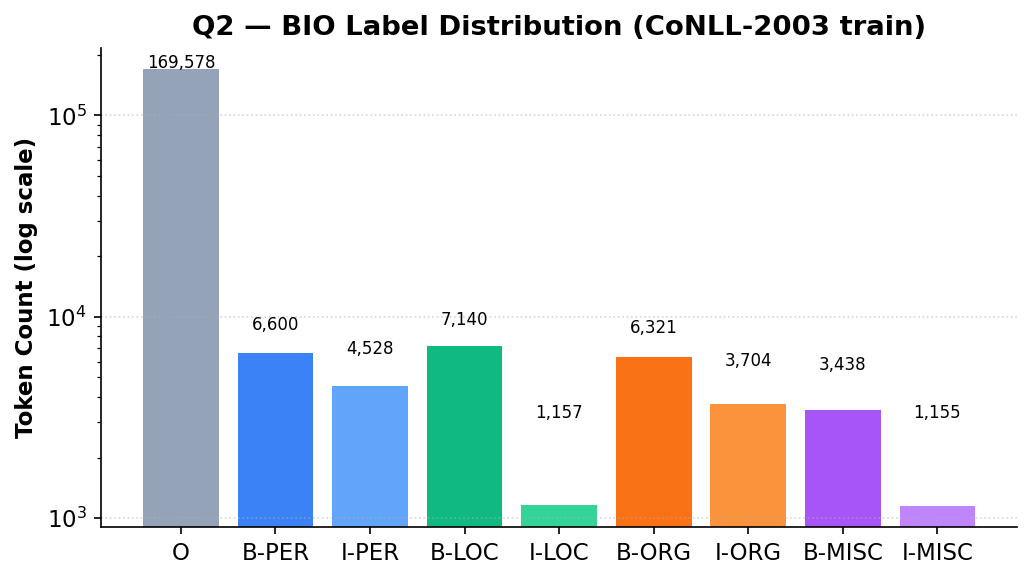
\includegraphics[width=0.78\textwidth]{figures/q2_label_dist.png}
\caption{BIO label distribution in the CoNLL-2003 training split (log scale). The \texttt{O} class dominates, motivating entity-level rather than token-level evaluation metrics.}
\label{fig:q2_dist}
\end{figure}

\subsection{Models}
\textbf{BiLSTM-CRF.} 128-dim embeddings $\rightarrow$ 2 BiLSTM layers (hidden 256/direction) $\rightarrow$ Conditional Random Field decoder~\cite{lafferty2001conditional}. The CRF globally normalises over label sequences, enforcing valid BIO transitions (e.g.\ \texttt{I-ORG} cannot follow \texttt{B-PER}) and decodes with Viterbi. Trained for 8 epochs (Adam, lr $10^{-3}$, batch 64, gradient clip 5.0, dropout 0.33).

\textbf{BERT Token Classifier.} A linear projection of dimension 9 is appended to \texttt{bert-base-cased}~\cite{devlin2019bert}, fine-tuned for 4 epochs (AdamW, lr $3{\times}10^{-5}$, batch 32, 10\% warmup). A CRF was deliberately omitted because BERT's self-attention already models long-range token interaction.

\subsection{Results}

\begin{table}[H]
\centering
\caption{Q2 Named Entity Recognition -- CoNLL-2003 test set.}
\label{tab:q2_overall}
\begin{tabular}{lccc}
\toprule
\textbf{Model} & \textbf{Precision} & \textbf{Recall} & \textbf{F1} \\
\midrule
BiLSTM-CRF (2L, hid=256) & 0.8180 & 0.6795 & 0.7424 \\
BERT (\texttt{bert-base-cased}, 4 ep) & \textbf{0.9035} & \textbf{0.9208} & \textbf{0.9121} \\
\bottomrule
\end{tabular}
\end{table}

\begin{table}[H]
\centering
\caption{Per-entity F1 scores on CoNLL-2003 test set.}
\label{tab:q2_entity}
\begin{tabular}{lcccc}
\toprule
\textbf{Model} & \textbf{PER} & \textbf{LOC} & \textbf{ORG} & \textbf{MISC} \\
\midrule
BiLSTM-CRF & 0.76 & 0.79 & 0.70 & 0.69 \\
BERT       & \textbf{0.96} & \textbf{0.93} & \textbf{0.89} & \textbf{0.80} \\
\bottomrule
\end{tabular}
\end{table}

\begin{figure}[H]
\centering
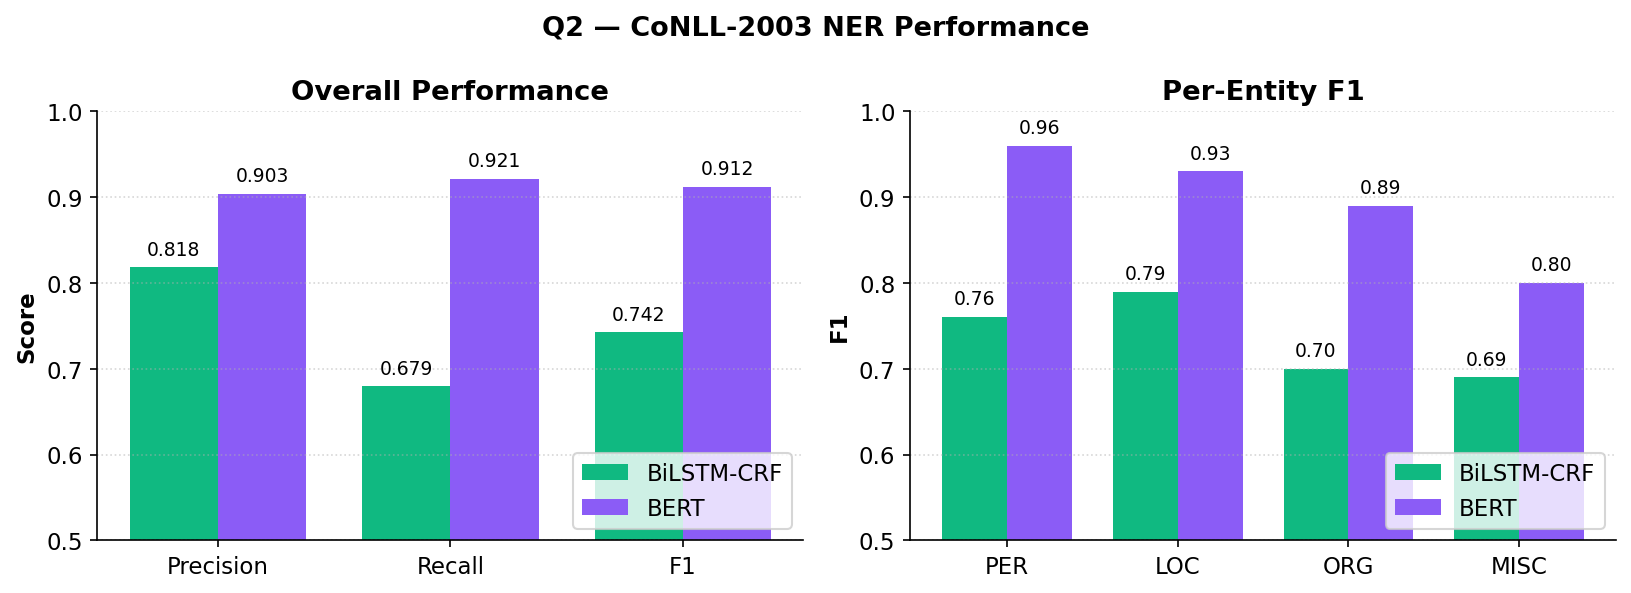
\includegraphics[width=0.95\textwidth]{figures/q2_ner.png}
\caption{Overall (left) and per-entity (right) NER scores. BERT improves F1 by nearly 17 absolute points overall and by 19+ points on PER and ORG.}
\label{fig:q2}
\end{figure}

BERT reaches an F1 of 91.21\%, 16.97 points above the BiLSTM-CRF (74.24\%). The BiLSTM-CRF's recall (0.6795) is its dominant weakness: it misses many entity mentions, while its precision (0.8180) shows that what it does predict is largely correct. BERT shows the opposite tilt: its recall (0.9208) slightly exceeds its precision (0.9035), the preferable trade-off in NER, where a missed entity is more costly downstream than a spurious one.

\subsection{Error Analysis and Discussion}
Two error families recur. The first is \emph{boundary mis-tagging on multi-token entities}: tokens such as ``World'' carry positional ambiguity (entity-initial in ``World Cup'' but entity-internal in ``FIFA World Cup''), and BERT occasionally emits \texttt{B-MISC} where \texttt{I-MISC} is correct. Hyphenated strings (``SKIING-WORLD'') exacerbate this. The second is \emph{type confusion on geopolitical/organizational ambiguity}: ``JAPAN'' is mis-tagged as \texttt{B-ORG} (national team) instead of \texttt{B-LOC} (country) by both models in sports-newswire context. The BiLSTM-CRF additionally fails on rare surnames (e.g.\ ``CUTTITTA'' $\rightarrow$ \texttt{B-LOC}): without strong contextual evidence, infrequent vocabulary defaults to common false-positive categories.

The performance gap is larger here than in sentiment classification because NER simultaneously requires \emph{precise span boundaries} and \emph{fine-grained type disambiguation}. BERT's pretrained embeddings already encode encyclopaedic knowledge about which surface forms are likely entity mentions, learned implicitly from co-occurrence in Wikipedia and BookCorpus. The BiLSTM-CRF must learn this from random initialisation. From a deployment standpoint, BiLSTM-CRF still has a niche: CPU inference is an order of magnitude faster, retraining on domain-specific entity types takes minutes, and it is preferable for high-throughput streaming pipelines where BERT's GPU latency is prohibitive.

%==============================================================================
\section{Question 3: Text Summarization}
%==============================================================================

\subsection{Dataset, Methods, and Metrics}
The CNN/DailyMail dataset is a large-scale summarization benchmark pairing news articles with human-written highlights. Articles average $\sim$800 tokens and references $\sim$55 tokens, giving a 14:1 compression ratio. Evaluation uses a random 500-example test subset (seed 42), with BERTScore on the first 200 examples.

\textbf{TextRank}~\cite{mihalcea2004textrank} is a graph-based extractive summariser: sentences are nodes, edge weights are cosine TF-IDF similarities, and PageRank scores select the top three sentences in document order. It cannot hallucinate because it copies sentences verbatim, but it is constrained to whole-sentence selection.

\textbf{BART}~\cite{lewis2020bart} is a pretrained denoising encoder--decoder transformer; the \texttt{bart-large-cnn} checkpoint has been further fine-tuned on the full CNN/DailyMail training set. We use it zero-shot with beam search (4 beams), output length bounded between 30 and 128 tokens.

Six metrics are reported: ROUGE-1/2/L for $n$-gram overlap, BLEU for $n$-gram precision, METEOR for stem/synonym alignment, and BERTScore-F1 for contextual semantic similarity.

\subsection{Results}

\begin{table}[H]
\centering
\caption{Q3 Text Summarization -- CNN/DailyMail (500 test samples). Scores on a 0--100 scale.}
\label{tab:q3}
\begin{tabular}{lcccccc}
\toprule
\textbf{Model} & \textbf{R-1} & \textbf{R-2} & \textbf{R-L} & \textbf{BLEU} & \textbf{METEOR} & \textbf{BERTScore-F1} \\
\midrule
TextRank (3 sentences) & 26.30 & 8.82 & 17.60 & 4.66 & 31.75 & 77.65 \\
BART (\texttt{bart-large-cnn}, ZS) & \textbf{35.82} & \textbf{15.33} & \textbf{26.47} & \textbf{12.15} & \textbf{32.69} & \textbf{80.62} \\
\bottomrule
\end{tabular}
\end{table}

\begin{figure}[H]
\centering
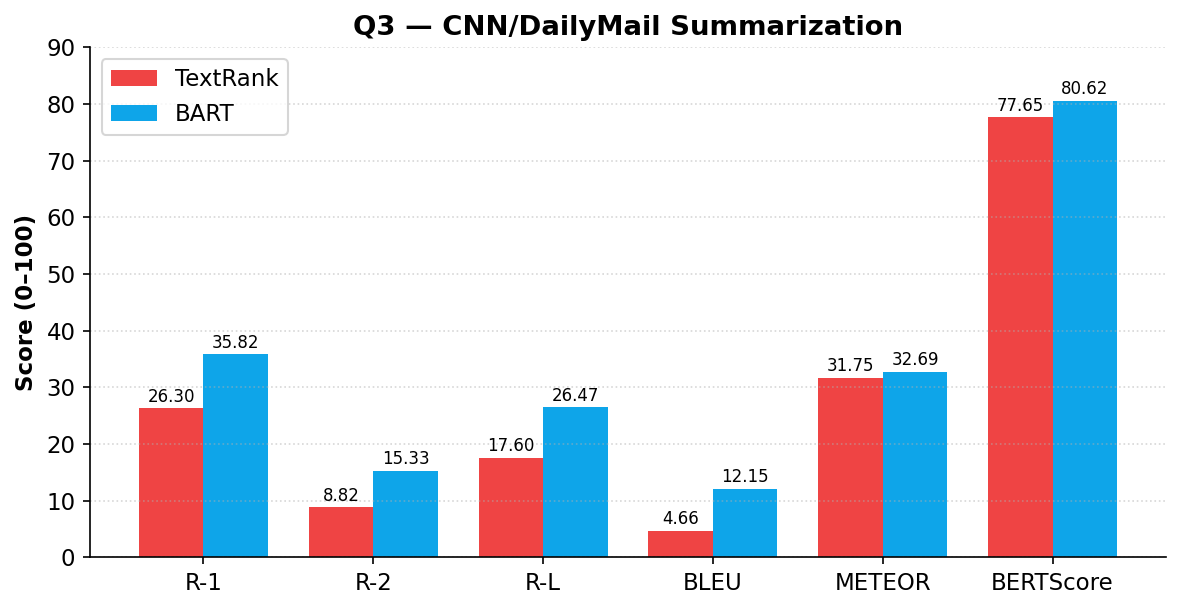
\includegraphics[width=0.83\textwidth]{figures/q3_summarization.png}
\caption{BART outperforms TextRank on every automatic metric. The gap is largest on ROUGE-2 and BLEU, which reward bigram-level content overlap.}
\label{fig:q3_metrics}
\end{figure}

\begin{figure}[H]
\centering
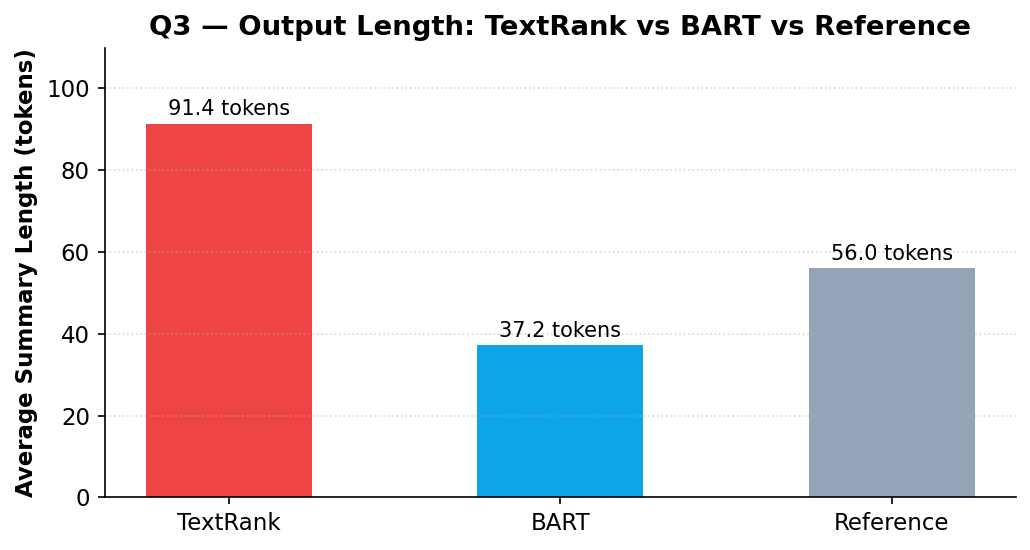
\includegraphics[width=0.62\textwidth]{figures/q3_length.png}
\caption{Average summary length: TextRank produces verbose 91-token extracts, while BART compresses to 37 tokens -- closer to the 56-token reference.}
\label{fig:q3_len}
\end{figure}

The ROUGE-2 gap (15.33 vs.\ 8.82) is especially telling: BART's generative capacity captures specific content phrases that TextRank, restricted to whole-sentence selection, often misses. METEOR scores are closest because METEOR rewards stems and synonyms in either output style. BERTScore confirms BART's semantic edge in contextual embedding space.

\subsection{Qualitative Analysis}

\begin{table}[H]
\centering
\caption{Representative qualitative findings from three test examples.}
\label{tab:q3_qual}
\small
\begin{tabular}{p{2.5cm}p{5.5cm}p{5.5cm}}
\toprule
\textbf{Example} & \textbf{TextRank behaviour} & \textbf{BART behaviour} \\
\midrule
Palestinian Authority / ICC (idx 0) & Selects a 76-word legal-background sentence; faithful but verbose. & Compact two-sentence summary of membership, jurisdiction, and US/Israel opposition. \\
\midrule
Andrew Getty death (idx 7) & Emphasises family statement and lineage. & Prioritises ``no foul play'' and health issues, matching the reference framing. \\
\midrule
Lynyrd Skynyrd drummer (idx 42) & Includes off-topic touring-history detail. & Concise two-sentence summary aligned with the main event. \\
\bottomrule
\end{tabular}
\end{table}

\subsection{Discussion}
The fundamental trade-off is precision vs.\ faithfulness. Extractive methods guarantee that every word appears in the source, eliminating hallucination -- a serious concern in legal, medical or financial domains. BART, despite better automatic scores, can introduce subtle factual distortions through paraphrasing, which automatic metrics do not capture. Latency differs by two orders of magnitude (TextRank $<$1\,ms vs.\ BART $\sim$200\,ms with beam search on GPU), making TextRank appealing for real-time, high-volume pipelines. BERTScore is the closest proxy to human judgment among the metrics used here, because it compares contextual embeddings and is robust to surface paraphrase.

%==============================================================================
\section{Question 4: Machine Translation}
%==============================================================================

\subsection{Dataset, Preprocessing, and Models}
The Multi30k dataset~\cite{elliott2016multi30k} pairs Flickr30k image captions with German translations: $\sim$29{,}000 training, 1{,}014 validation, and 1{,}000 test pairs. Captions average 12--13 tokens and describe everyday visual scenes. The vocabulary is approximately 10k English types versus 18k German types -- the larger German vocabulary reflects morphological richness.

For Seq2Seq, text is lowercased, tokenized with SpaCy, with words below frequency 2 mapped to \texttt{<UNK>}, padded to 50 tokens with \texttt{<sos>}/\texttt{<eos>} markers. MarianMT uses its native SentencePiece tokenizer with a $\sim$65k subword vocabulary, structurally eliminating OOV tokens.

\textbf{Seq2Seq with Bahdanau attention}~\cite{bahdanau2015neural}. BiGRU encoder (2L, hidden 512) $+$ unidirectional GRU decoder (2L, hidden 512) $+$ MLP additive attention. Embedding 256, dropout 0.3, teacher forcing 0.5, 15 epochs (Adam, lr $5{\times}10^{-4}$, batch 128, gradient clip 1.0).

\textbf{MarianMT}~\cite{tiedemann2020opus}. Production-grade transformer (\texttt{Helsinki-NLP/opus-mt-en-de}) trained on the OPUS corpus with 6+6 encoder/decoder layers and multi-head self/cross-attention, used zero-shot.

\subsection{Results}

\begin{table}[H]
\centering
\caption{Q4 Machine Translation -- Multi30k EN$\rightarrow$DE test set (1{,}000 samples). Scores on a 0--100 scale.}
\label{tab:q4}
\begin{tabular}{lcccc}
\toprule
\textbf{Model} & \textbf{BLEU} & \textbf{METEOR} & \textbf{ChrF} & \textbf{BERTScore-F1} \\
\midrule
Seq2Seq + Bahdanau Attention & 26.16 & 56.14 & 53.09 & 91.93 \\
MarianMT (Helsinki-NLP, ZS) & \textbf{36.37} & \textbf{66.55} & \textbf{64.23} & \textbf{94.30} \\
\bottomrule
\end{tabular}
\end{table}

\begin{figure}[H]
\centering
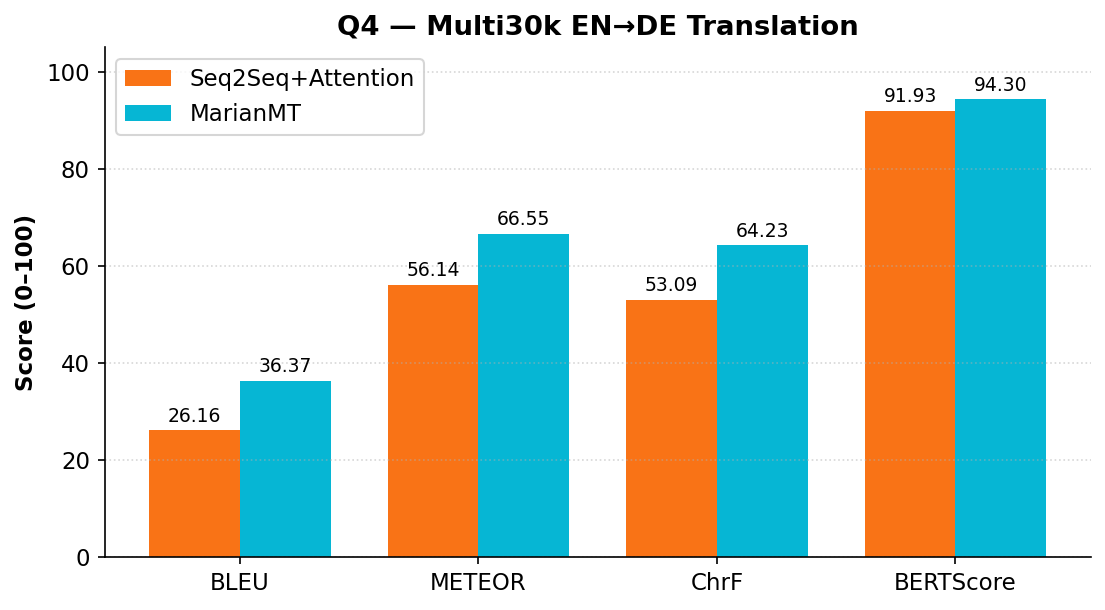
\includegraphics[width=0.78\textwidth]{figures/q4_translation.png}
\caption{Multi30k EN$\rightarrow$DE results. The BLEU gap (+10.21) is the largest; ChrF (+11.14) confirms MarianMT's superior handling of German morphology at the character level.}
\label{fig:q4_metrics}
\end{figure}

\begin{figure}[H]
\centering
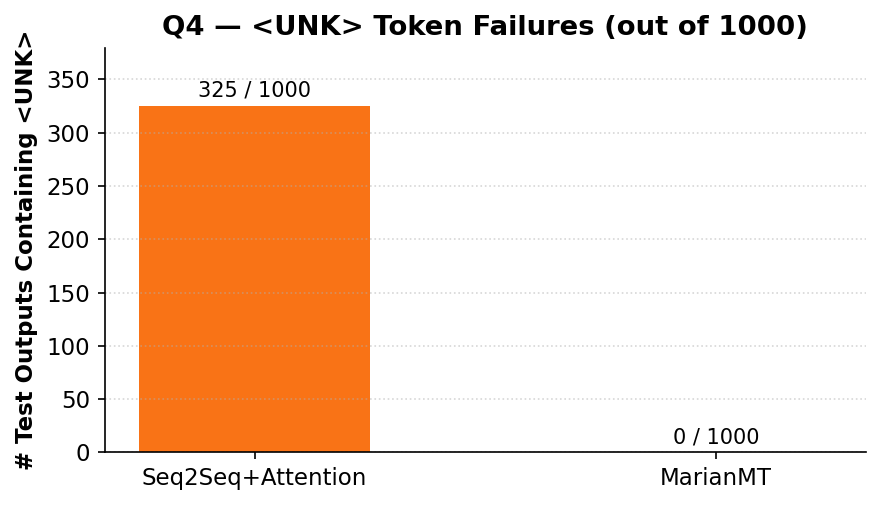
\includegraphics[width=0.55\textwidth]{figures/q4_unk.png}
\caption{Vocabulary coverage failure. 325 of the 1{,}000 Seq2Seq outputs contain at least one \texttt{<UNK>} token; MarianMT produces zero, owing to SentencePiece subword decomposition.}
\label{fig:q4_unk}
\end{figure}

\subsection{Qualitative Analysis}

\begin{table}[H]
\centering
\caption{Translation example illustrating rare-word and morphology behaviour.}
\label{tab:q4_qual}
\small
\begin{tabular}{lp{11cm}}
\toprule
Source     & a young boy in a soccer uniform crying into his palms \\
Reference  & Ein kleiner Junge im Fußballdress hält die Hände vors Gesicht und weint. \\
Seq2Seq    & ein kleiner junge in einem fußballtrikot in in sein \texttt{<unk>} \\
MarianMT   & Ein kleiner Junge in einer Fußballuniform, der in seine Handflächen weint. \\
\bottomrule
\end{tabular}
\end{table}

The Seq2Seq output combines repetition (``in in'') with an \texttt{<unk>} token for the crucial content word ``palms''. MarianMT produces a fluent, faithful translation through SentencePiece subword decomposition. GRU \emph{attention collapse} is the recurring failure mode: when source content is rare or alignment is non-monotonic (typical in English--German verb-final constructions), the soft attention distribution becomes diffuse, and the decoder falls back on high-frequency function words or repeats earlier output. This pathology is most severe for sentences longer than 20 tokens and is structural -- recurrent hidden-state distortion accumulates with sequence length. Transformer cross-attention does not suffer this: scaled dot-product attention with positional encoding accesses any source position in $O(1)$ steps without recurrent distortion.

\subsection{Discussion}
The four metrics are complementary. BLEU is fluent-but-strict; METEOR rewards stems and synonyms; ChrF is robust to morphology and tokenisation, especially valuable for German where \emph{Hut} vs.\ \emph{Hutes} would score zero under BLEU but positive under ChrF; BERTScore evaluates contextual semantic similarity. Seq2Seq + attention remains \emph{viable} for short, in-domain captions when training data is dense relative to vocabulary, but its three structural weaknesses -- fixed vocabulary, sequential hidden-state accumulation and attention collapse on long/rare inputs -- make it unsuitable for open-domain deployment. MarianMT's three cumulative advantages (massive multilingual pretraining on OPUS, SentencePiece OOV elimination, and global transformer attention) compound to produce a $\sim$10 BLEU advantage zero-shot. The practical takeaway is unambiguous: pretrained transformer MT should be the default choice in production.

%==============================================================================
\section{Question 5: Language Modeling}
%==============================================================================

\subsection{Dataset and Models}
WikiText-2~\cite{merity2017pointer} is a word-level language modeling benchmark of curated Wikipedia ``Good and Featured'' articles, with $\sim$2.1M training tokens, 217k validation tokens and 245k test tokens over a $\sim$33k-type vocabulary. Whitespace word-level tokenisation is used. The trigram model is evaluated on the first 5{,}000 test tokens with Laplace smoothing $\alpha{=}0.1$; the LSTM uses BPTT length 35.

\textbf{Trigram} estimates $P(w_t \mid w_{t-2}, w_{t-1})$ with Laplace smoothing. Smoothing is essential because the trigram context space has $|V|^2 \approx 10^9$ possible histories, of which the corpus contains only $\sim$700k distinct trigrams; without smoothing, most test contexts receive zero probability.

\textbf{LSTM Language Model.} 512-dim embedding $\rightarrow$ 2-layer LSTM (hidden 512, dropout 0.35) $\rightarrow$ output projection. \emph{Weight tying}~\cite{merity2017pointer} binds the embedding matrix to the output projection, removing $\sim$17M parameters and acting as a regulariser. Trained 15 epochs with SGD (lr $5{\times}10^{-3}$), BPTT 35; SGD is preferred over Adam for this benchmark because it generalises better in this regime.

\subsection{Results}

\begin{table}[H]
\centering
\caption{Q5 Language Modeling -- WikiText-2 test set.}
\label{tab:q5}
\begin{tabular}{lccp{4.0cm}}
\toprule
\textbf{Model} & \textbf{Val PPL} & \textbf{Test PPL} & \textbf{Notes} \\
\midrule
3-gram (Laplace $\alpha{=}0.1$) & 5317.49 & 5491.11 & No GPU, fast \\
LSTM (2L, hid=512, tied) & \textbf{1415.95} & \textbf{1330.83} & BPTT, weight tying \\
\bottomrule
\end{tabular}
\end{table}

\begin{figure}[H]
\centering
\begin{minipage}{0.46\textwidth}
\centering
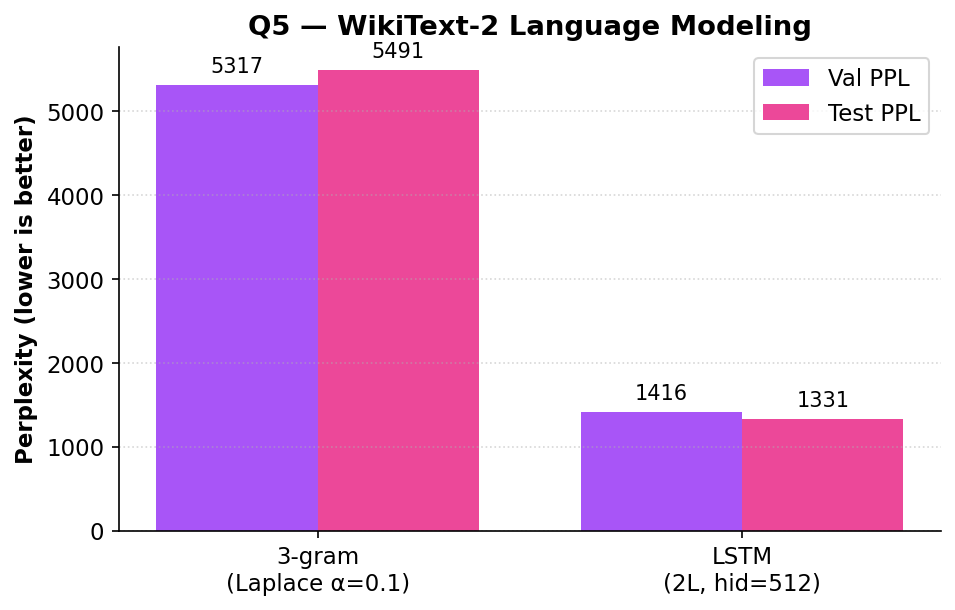
\includegraphics[width=\textwidth]{figures/q5_lm.png}
\end{minipage}\hfill
\begin{minipage}{0.50\textwidth}
\centering
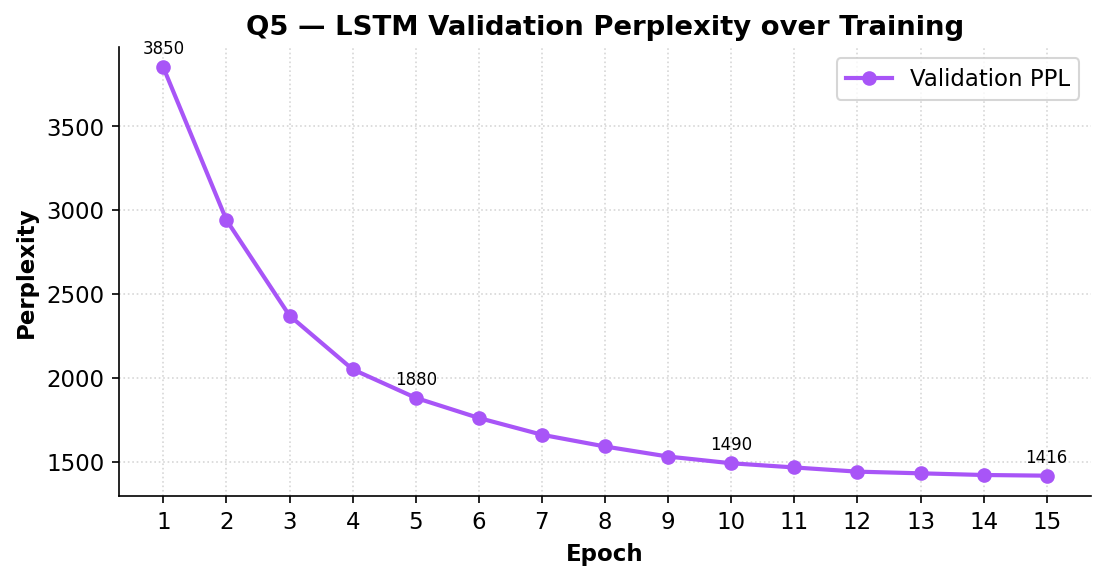
\includegraphics[width=\textwidth]{figures/q5_lstm_curve.png}
\end{minipage}
\caption{Left: Validation/test perplexity comparison. The LSTM reduces test PPL by 4.1$\times$. Right: LSTM validation perplexity over 15 training epochs, showing steady descent without plateau.}
\label{fig:q5}
\end{figure}

\subsection{Generated Text Samples and Discussion}
\textbf{Seed: ``the history of''.} \emph{Trigram}: ``the history of the hnc as decision no. 1 squadron was sent back to north america.'' Locally fluent because trigrams literally copy three-word sequences from training, but topical drift (history $\rightarrow$ squadrons $\rightarrow$ computer programs) reveals zero global coherence. \emph{LSTM}: ``the history of woodland takeda cpr johnston in the , moniteur an this \texttt{<unk>} itcz 1905\ldots''. Lexically diverse, locally syntactic, but semantically incoherent. The two failure modes are qualitatively different: the trigram \emph{copies} fragments, the LSTM \emph{generalises} but lacks topic persistence.

Perplexity is $2^{H(p,q)}$, the exponential of cross-entropy between true and model distributions. The trigram model's high PPL is a direct \emph{sparsity} consequence: $|V|^2 \approx 10^9$ contexts exist, the training corpus covers a tiny fraction, and Laplace smoothing redistributes 0.1 mass uniformly to every unobserved continuation. With a 33k vocabulary this spreads the smoothed mass extremely thinly, producing tiny probabilities and correspondingly large cross-entropy.

The LSTM avoids this curse of dimensionality by mapping any context into a continuous 512-dimensional hidden state. Words playing similar grammatical or semantic roles receive similar hidden representations, so probability mass generalises smoothly across lexically distinct but structurally equivalent contexts. This is exactly the advantage of distributed neural representations over discrete $n$-gram tables: an exponential number of histories collapses into a manageable continuous manifold. The remaining gap between our LSTM ($\sim$1330) and state-of-the-art transformer LMs on WikiText-2 ($\sim$60--80) reflects three further factors: a short BPTT window (35 tokens), the absence of advanced regularisation (variational dropout, AR/TAR), and the fundamental superiority of transformer self-attention over recurrent compression for very long-range dependencies.

%==============================================================================
\section{Conclusion}
%==============================================================================

This investigation systematically compared classical, recurrent and transformer-based approaches across five canonical NLP tasks. Several cross-task lessons emerge.

\textbf{Transformer dominance is consistent and substantial.} Pretrained transformers (DistilBERT, BERT, BART, MarianMT) win every task, with absolute gaps ranging from $\sim$1.4 points (sentiment) to nearly 17 points (NER) and 10 BLEU (MT). The gap is largest on tasks that require precise local decisions integrated with global context (NER, MT), and smaller on tasks where bag-of-words signal is already strong (sentiment classification).

\textbf{Data efficiency favours simple inductive biases.} Models trained from scratch (BiLSTM for IMDb/NER, Seq2Seq for MT) systematically underperform classical baselines (TF-IDF LR, $n$-gram LM, TextRank) when training data is limited relative to vocabulary. The 89.74\% bigram TF-IDF score on IMDb illustrates this clearly: a problem-matched inductive bias (bag of phrases for document-level sentiment) compensates for a complete lack of contextual modelling.

\textbf{Vocabulary coverage is a first-order design choice.} Multi30k Seq2Seq emitted 325 \texttt{<unk>} tokens in 1{,}000 outputs, while MarianMT emitted zero. The trigram LM's 5491 perplexity is essentially a vocabulary-coverage failure. Subword tokenisation (SentencePiece, WordPiece) addresses this structurally for neural models; smoothed back-off addresses it probabilistically for $n$-gram models, but neither is a complete solution.

\textbf{Classical models are not obsolete.} TF-IDF LR, $n$-gram LMs, TextRank and BiLSTM-CRF all retain practical niches: when interpretability, CPU deployment, hard latency budgets or guaranteed faithfulness are required, they are often better engineering choices than transformer alternatives. The optimal architecture for any production NLP system must explicitly balance accuracy, latency, interpretability and infrastructure cost.

\textbf{Evaluation matters as much as modelling.} The four MT metrics, six summarisation metrics and entity-level NER scores collectively show that no single number captures task quality. Reporting multiple, complementary metrics is essential to draw defensible conclusions about model behaviour.

\bibliographystyle{plain}
\begin{thebibliography}{11}

\bibitem{maas2011learning}
A.~L. Maas, R.~E. Daly, P.~T. Pham, D.~Huang, A.~Y. Ng, and C.~Potts.
\newblock Learning word vectors for sentiment analysis.
\newblock In \emph{Proceedings of ACL}, pages 142--150, 2011.

\bibitem{tjong2003introduction}
E.~F. Tjong Kim~Sang and F.~De~Meulder.
\newblock Introduction to the CoNLL-2003 shared task: Language-independent named entity recognition.
\newblock In \emph{Proceedings of CoNLL}, pages 142--147, 2003.

\bibitem{devlin2019bert}
J.~Devlin, M.-W. Chang, K.~Lee, and K.~Toutanova.
\newblock {BERT}: Pre-training of deep bidirectional transformers for language understanding.
\newblock In \emph{Proceedings of NAACL-HLT}, pages 4171--4186, 2019.

\bibitem{sanh2019distilbert}
V.~Sanh, L.~Debut, J.~Chaumond, and T.~Wolf.
\newblock {DistilBERT}, a distilled version of {BERT}: smaller, faster, cheaper and lighter.
\newblock In \emph{EMC$^2$ Workshop at NeurIPS}, 2019.

\bibitem{bahdanau2015neural}
D.~Bahdanau, K.~Cho, and Y.~Bengio.
\newblock Neural machine translation by jointly learning to align and translate.
\newblock In \emph{Proceedings of ICLR}, 2015.

\bibitem{lewis2020bart}
M.~Lewis, Y.~Liu, N.~Goyal, M.~Ghazvininejad, A.~Mohamed, O.~Levy, V.~Stoyanov, and L.~Zettlemoyer.
\newblock {BART}: Denoising sequence-to-sequence pre-training for natural language generation, translation, and comprehension.
\newblock In \emph{Proceedings of ACL}, pages 7871--7880, 2020.

\bibitem{lafferty2001conditional}
J.~Lafferty, A.~McCallum, and F.~C.~N. Pereira.
\newblock Conditional random fields: Probabilistic models for segmenting and labeling sequence data.
\newblock In \emph{Proceedings of ICML}, pages 282--289, 2001.

\bibitem{mihalcea2004textrank}
R.~Mihalcea and P.~Tarau.
\newblock {TextRank}: Bringing order into texts.
\newblock In \emph{Proceedings of EMNLP}, pages 404--411, 2004.

\bibitem{elliott2016multi30k}
D.~Elliott, S.~Frank, K.~Sima'an, and L.~Specia.
\newblock {Multi30K}: Multilingual {English-German} image descriptions.
\newblock In \emph{Proceedings of the 5th Workshop on Vision and Language}, pages 70--74, 2016.

\bibitem{merity2017pointer}
S.~Merity, C.~Xiong, J.~Bradbury, and R.~Socher.
\newblock Pointer sentinel mixture models.
\newblock In \emph{Proceedings of ICLR}, 2017.

\bibitem{tiedemann2020opus}
J.~Tiedemann and S.~Thottingal.
\newblock {OPUS-MT} -- Building open translation services for the world.
\newblock In \emph{Proceedings of EAMT}, 2020.

\end{thebibliography}

\end{document}
